\documentclass[tikz,border=2pt]{standalone}
\usepackage{amsmath,amssymb}
\usepackage{tikz}
\usetikzlibrary{arrows.meta}

\begin{document}
% The range of A = [[1,2],[2,4]] is the line spanned by (1,2): every input lands on it.
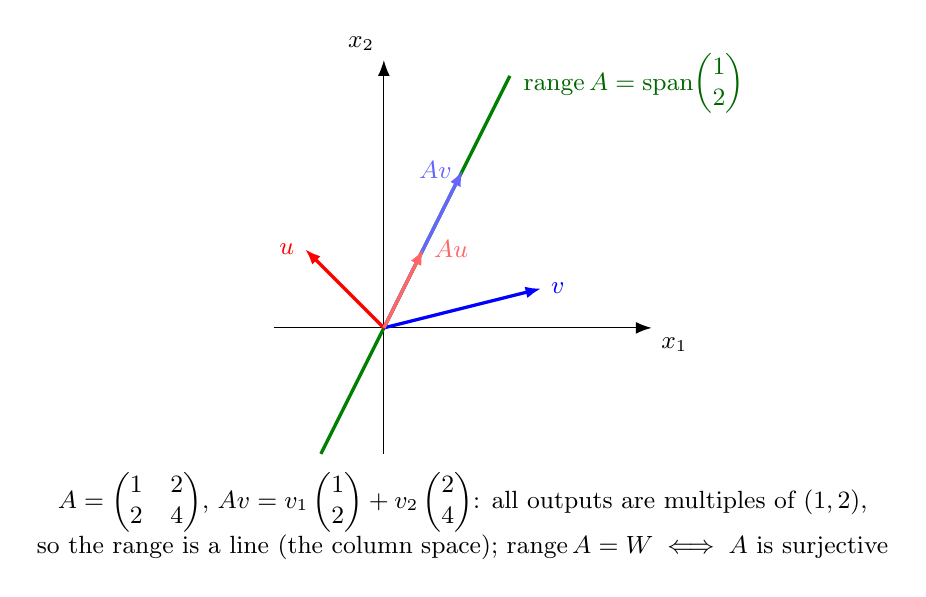
\begin{tikzpicture}[every node/.style={font=\small}, >={Latex[length=2mm]}]
	\draw[->] (-1.4,0) -- (3.4,0) node[below right] {$x_1$};
	\draw[->] (0,-1.6) -- (0,3.4) node[above left] {$x_2$};
	\draw[green!50!black, very thick] (-0.8,-1.6) -- (1.6,3.2);
	\node[green!40!black, anchor=west] at (1.65,3.1) {$\operatorname{range}A=\operatorname{span}\!\begin{pmatrix}1\\2\end{pmatrix}$};
	\draw[->, blue, very thick] (0,0) -- (2.0,0.5);
	\node[blue, right] at (2.0,0.5) {$v$};
	\draw[->, blue!60, very thick] (0,0) -- (1.0,2.0) node[left, font=\small] {$Av$};
	\draw[->, red, very thick] (0,0) -- (-1.0,1.0) node[left] {$u$};
	\draw[->, red!60, very thick] (0,0) -- (0.5,1.0) node[right, font=\small] {$Au$};
	\node[anchor=north, align=center] at (1,-1.7) {$A=\begin{pmatrix}1&2\\2&4\end{pmatrix}$, $Av=v_1\begin{pmatrix}1\\2\end{pmatrix}+v_2\begin{pmatrix}2\\4\end{pmatrix}$: all outputs are multiples of $(1,2)$,\\ so the range is a line (the column space); $\operatorname{range}A=W\iff A$ is surjective};
\end{tikzpicture}
\end{document}
